\documentclass[12pt]{article}
\usepackage[utf8]{inputenc}
\usepackage[norsk]{babel}
\usepackage[usenames,dvipsnames]{xcolor}
\usepackage{lmodern}
\usepackage[a4paper, margin=0.75in]{geometry}
\usepackage{lastpage}
\usepackage{fancyhdr}
\usepackage{parskip}
\usepackage{titlesec} 
\usepackage[T1]{fontenc}
\usepackage[pdftex]{graphicx}
\usepackage[none]{hyphenat}
\usepackage{lastpage}

\begin{document}
\pagestyle{fancy}
\fancyhf{}
\fancyhead[L]{\textit{Vedlegg til KS-beretning}}

\section*{Utleie våren 2016}
\label{sec:1}
\subsection*{Generelt}
Realistforeningen har som vanlig hatt utleier dette semesteret, se tabell under.
Standardlønnen dette semesteret har vært 144 kr i timen. 

For at flere skal få nytte av å jobbe betalt for RF,
har vi dette semesteret fortsatt med å gjøre det slik at de som ikke har jobbet,
men som ønsker det, stiller først i køen når nye jobber lyses ut.

All utleieutlysning går nå gjennom moneymaker@rf.uio.no først,
så alle som har lyst til å ha mulighet til å jobbe betalt for RF bør
melde seg på denne e-postlisten.

Vi har for fullt begynt med nettskjema for å registrere utleier:
http://utleieskjema.realistforeningen.no.

\subsection*{Arrangementer}
Realistforeningen har hatt eller planlegger følgende utleier våren 2016:\\

\begin{tabular}{l r}
\bfseries Arrangement & \bfseries Tid\\
\hline
Spillkveld, Ares &	Hver tirsdag\\
Eplefest, Matematisk institutt &	30.1.2016\\
Biørneball-nachspiel, Biørnegildet 2016 &	20.2.2016\\
Bedriftspresentasjon, Bekk &	24.2.2016\\
Quiz, Tekna & 25.2.2016\\
Quiz, Norsk selskap for immunologi &	2.3.2016\\
Foredragskveld 1, Norsk kristlig studentlag &	8.3.2016\\
Foredragskveld 2, Norsk kristlig studentlag &	9.3.2016\\
Foredragskveld 3, Norsk kristlig studentlag &	10.3.2016\\
Barnebursdag &	9.4.2016\\
Grønn pils, SP:UiO &	25.5.2016
\end{tabular}
\subsection*{Studentkjellernes personalforening}
Alle kjellerforeninger som har lyst til å utleier med utbetaling av lønn
må være med i Studentkjellernes personalforening (SPF).
RFs representant i SPF har vært utleiesjef.

\newpage

\begin{figure}[!ht]
  \centering
      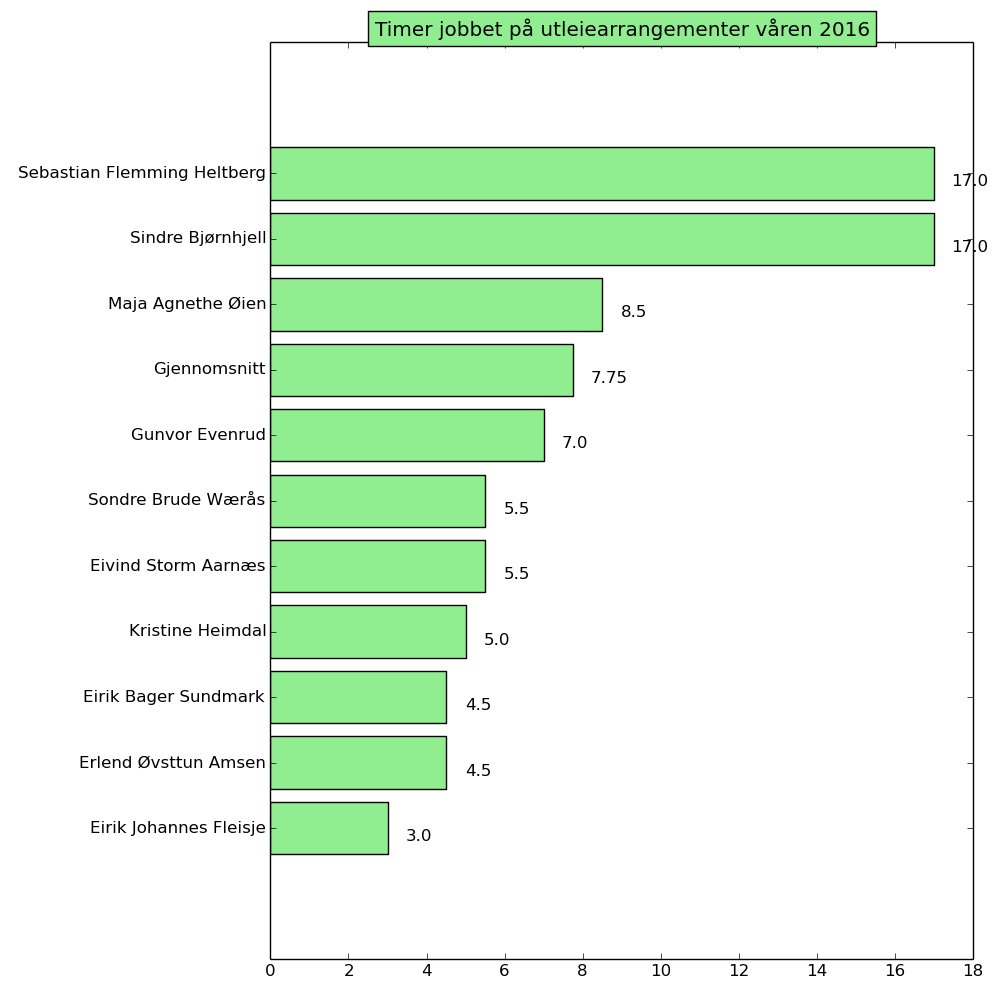
\includegraphics[width=1.0\textwidth]{utleiebar-V16.png}
  \caption{Oversikt over de som har jobbet på utleiearrangementer 
      dette semesteret}
\end{figure}
\end{document}
